  % this file is called up by thesis.tex
% content in this file will be fed into the main document
% ----------------------- name of chapter  -------------------------
%\newgeometry{top=-0.4cm, left=0.9cm, right=1.5cm}
\chapter{Charm tagging using DL1r}
\label{appendix:DL1rc}
% ----------------------- paths to graphics ------------------------

% change according to folder and file names
\ifpdf
    \graphicspath{Appendices/AP3/figures/}
\else
    \graphicspath{Appendices/AP3/figures/}
\fi
\vspace{-0.5cm}
% ----------------------- contents from here ------------------------
The DL1r tagger gives the probability a jet is a $b$-jet, $p_b$, $c$-jet, $p_c$, or light jet, $p_{light}$. 
Using these probabilities the discriminant variable can be constructed to discriminate a jet of type $i$ from jets of types $j$ and $k$:
\begin{equation}
\text{DL1r}_{i}=\ln\frac{p_i}{f_j\cdot p_j + (1 - f_j)\cdot p_k},
\end{equation}  
where the $f_j$ parameter controls whether jets of type $i$ are to be primarily discriminated from jets
of type $j$ or type $k$. In the specific case of $c$-tagging the discriminant becomes:
\begin{equation}
\text{DL1r}_{c}=\ln\frac{p_c}{f_b\cdot p_b + (1 - f_b)\cdot p_{light}}.
\end{equation}
A value of DL1r$_c$ must be chosen to cut on to decide whether a jet is a tagged as a $c$-jet or not.
Therefore, there are two parameters which must be chosen, the value of $f_b$ and the cut value, 
to have an optimal performance.\\
In order to determine the best values for $f_b$ and DL1r$_c$ cut, events are
selected using the SR1 selection described in~\cref{sec:other_selection}, excluding the FCNC top mass requirement. So, the selection is: 3 leptons,
$Z$ boson mass window, at least 2 jets with exactly one being $b$-tagged.
Then, several values for $f_b$ and DL1r$_c$ cut were considered and for each of them events are split into two categories, $c$-tagged events (=1 $c$-tag) and $c$-tag veto events.
The $c$-tagging is applied on jets that fail the $b$-tagging requirement.
For each combination of $f_b$ and DL1r$_c$ cut values, the $S/\sqrt{B}$ values were calculated in both $c$-tagged and $c$-tag veto events.
The optimal values for $f_b$ and DL1r$_c$ cut would be the ones that give highest value of $S/\sqrt{B}$ combined in quadrature from $c$-tagged and $c$-tag veto events.
\noindent \Cref{app:DL1rc:fig:SoverSqrtB} presents the $S/\sqrt{B}$ values for different $f_b$ and DL1r$_c$ cut values in $c$-tagged and $c$-tag veto events,
while combined $S/\sqrt{B}$ values are presented in~\cref{app:DL1rc:fig:SoverSqrtB_combined}.\\
%\restoregeometry
\noindent As the~\cref{app:DL1rc:fig:SoverSqrtB_combined} suggests, the optimal $c$-tagging working point (WP) would be at 0.6 for $f_b$ and 1.84 for DL1r$_c$ cut, which gives
highest value of 3.42 for combined $S/\sqrt{B}$. 
However, the optimal $c$-tagging working point must be calibrated, which is not trivial.
\noindent Alternatively, the $c$-tagging working point ($f_b=0.28$, DL1r$_c$ cut= 1.32) being calibrated in the $tc$+MET SUSY analysis~\cite{ANA-SUSY-2019-23} is used in this analysis.\\
\Cref{app:DL1rc:tab:WPs} summarises the performance of the considered $c$-tagging working points. 

\begin{figure}[htbp]
	\centering
	\begin{tabular}{cc}
		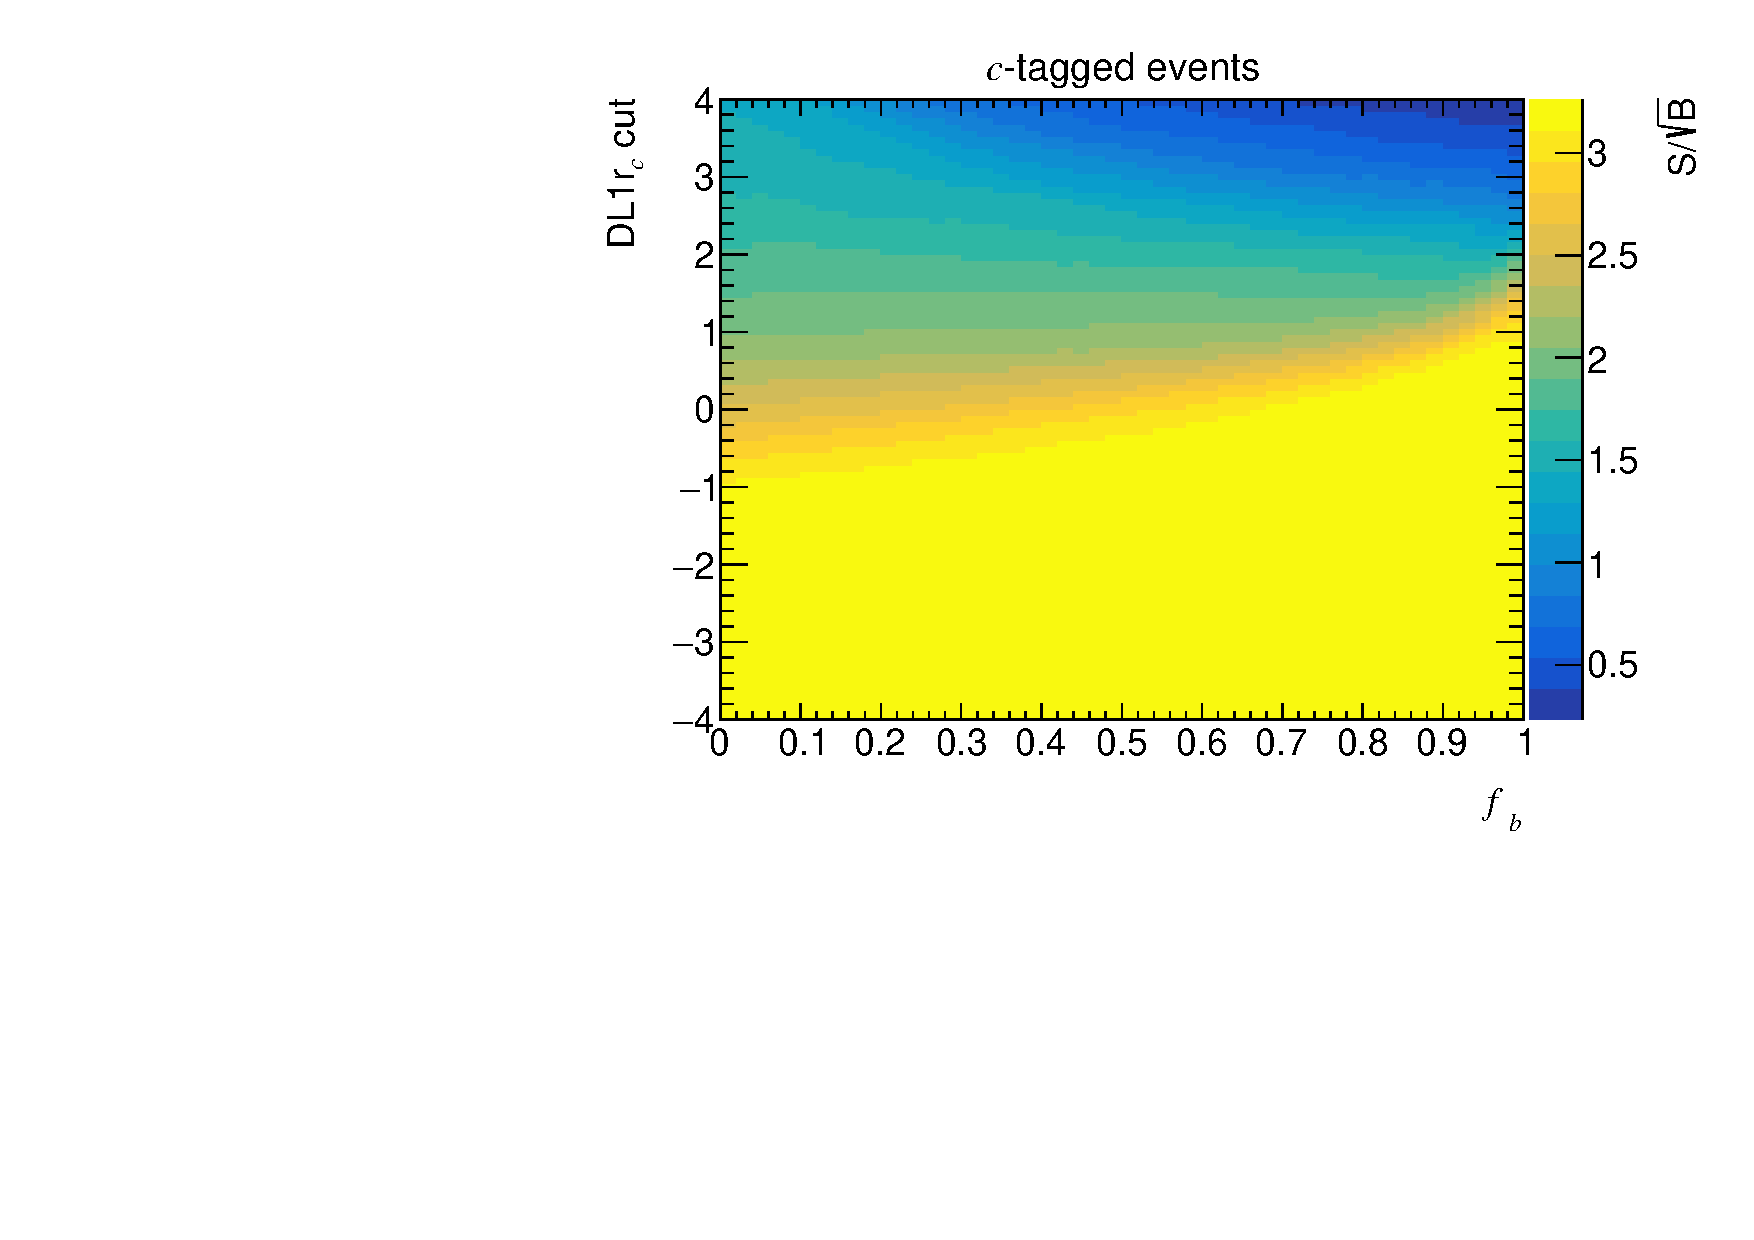
\includegraphics[width=.42\textwidth]{Appendices/AP3/figures/c-tagged} &
		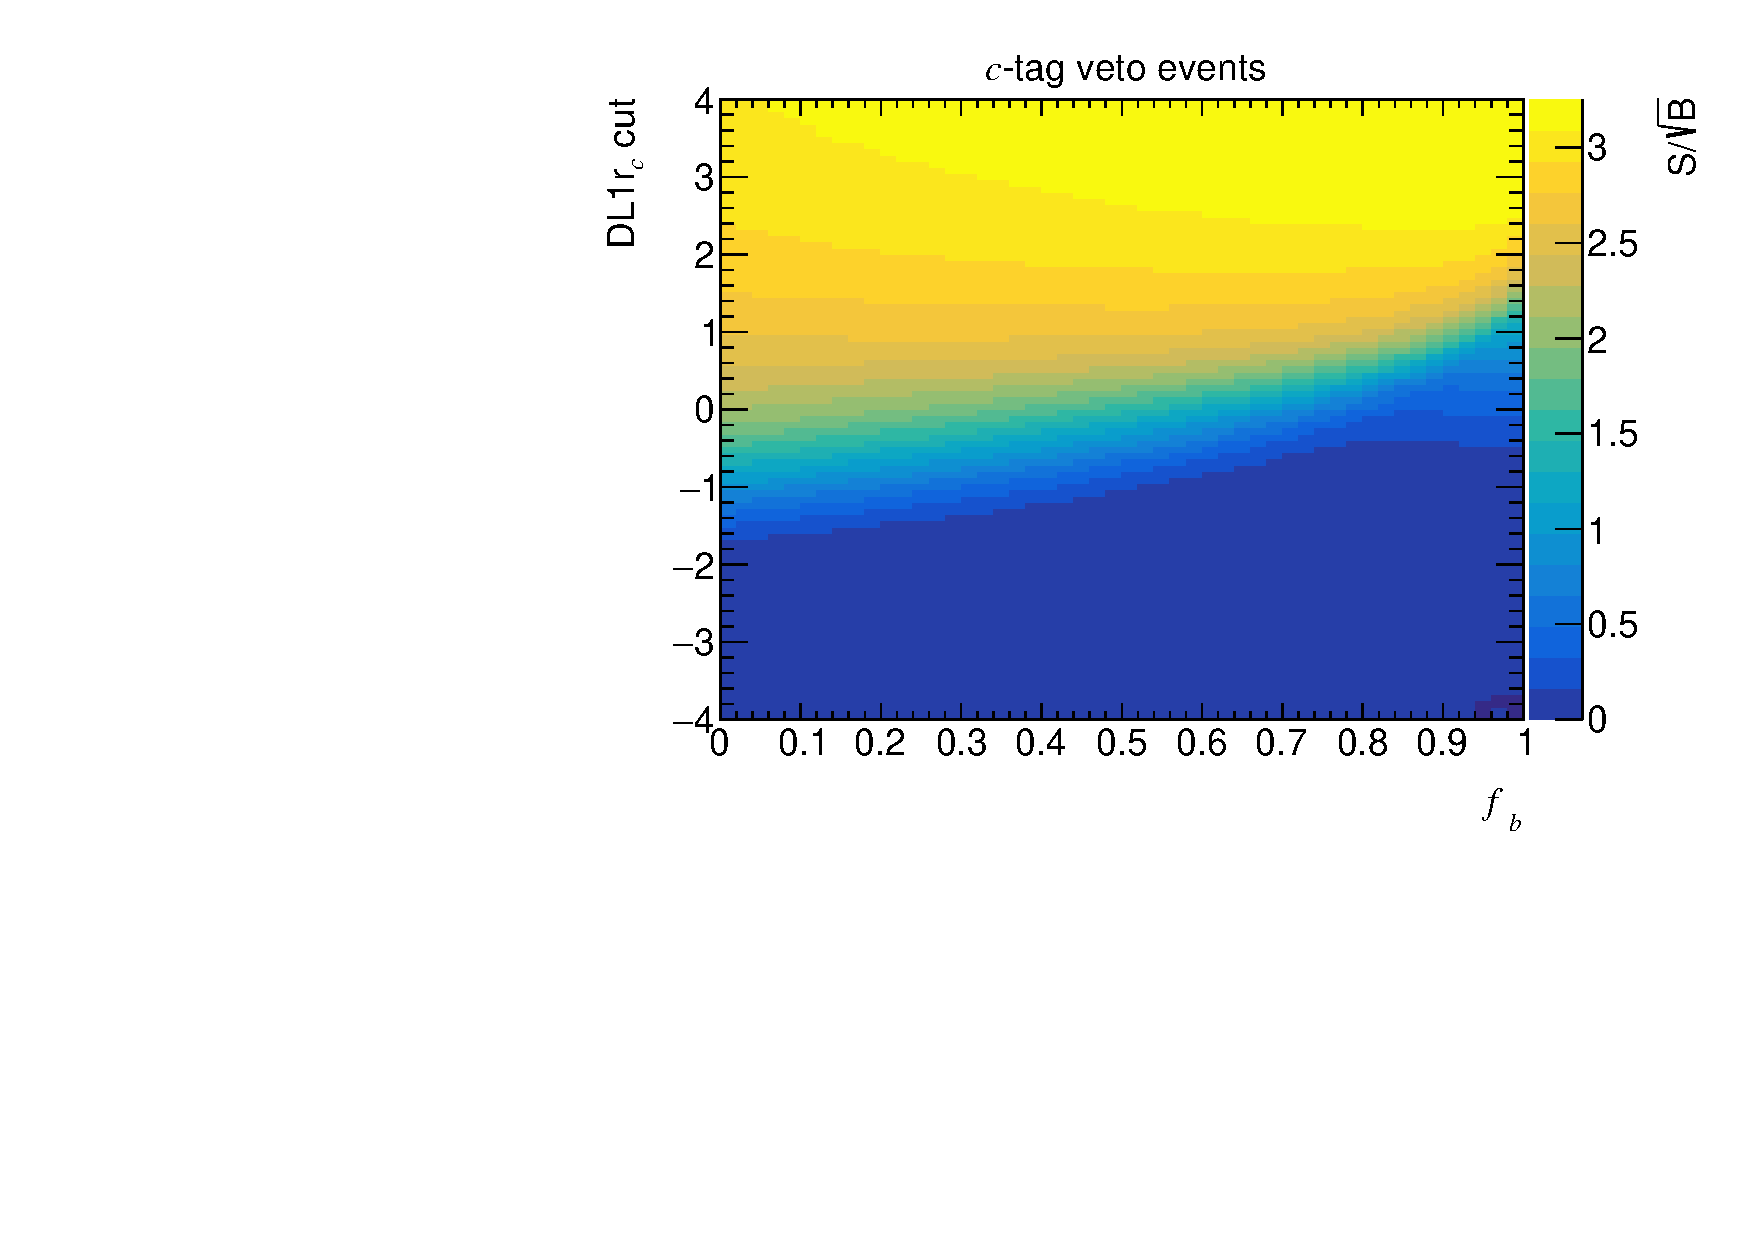
\includegraphics[width=.42\textwidth]{Appendices/AP3/figures/c-tag_veto}
	\end{tabular}
	\caption{ The $S/\sqrt{B}$ values for different $f_b$ and DL1r$_c$ cut values in $c$-tagged (left) and $c$-tag veto (right) events. }
	\label{app:DL1rc:fig:SoverSqrtB}
\end{figure}
\begin{figure}[htbp]
	\centering
	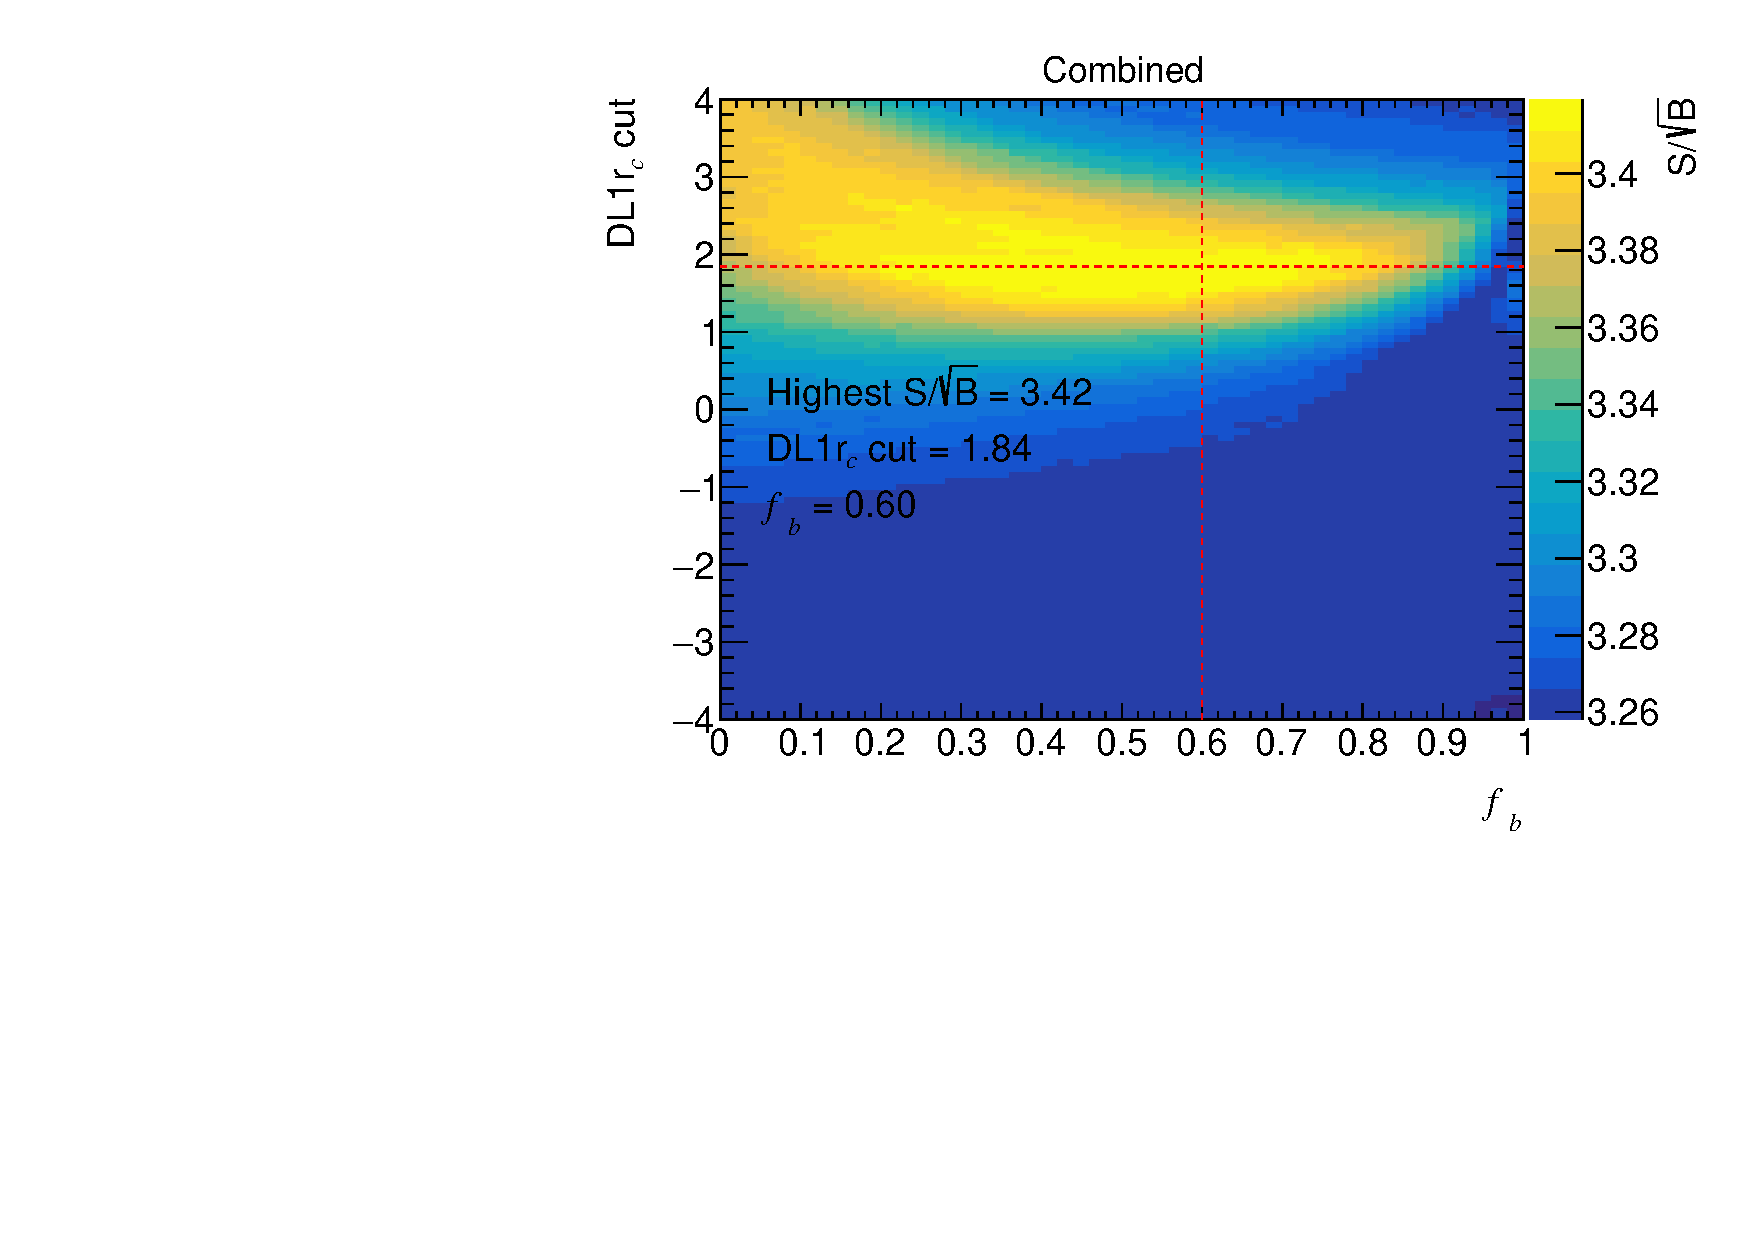
\includegraphics[width=.43\textwidth]{Appendices/AP3/figures/Combined}
	\caption{ The $S/\sqrt{B}$ values combined in quadrature from $c$-tagged and $c$-tag veto events for different $f_b$ and DL1r$_c$ cut values.
		The vertical and horizontal dashed lines indicate the $f_b$ and DL1r$_c$ cut values which give highest $S/\sqrt{B}$ value. }
	\label{app:DL1rc:fig:SoverSqrtB_combined}
\end{figure}
\vspace{-0.3cm}
\begin{table}[!htbp]
	\small
	\centering
	\begin{tabular}{l|cc|cc}
		\toprule
		& $f_b=0.28$ & DL1r$_c$ cut & $S/\sqrt{B}$ & \BR($t\to Zc$) limit  \\
		\midrule
		Optimal WP & 0.6 & 1.84 & 3.42 & $9.5\times 10^{-5}$ \\
		$tc$+MET SUSY WP & 0.28 & 1.32 & 3.39 & $9.7\times 10^{-5}$ \\
		\bottomrule
	\end{tabular}
	\label{app:DL1rc:tab:WPs}
	\caption{
		\small{
		Combined $S/\sqrt{B}$ values from $c$-tagged and $c$-tag veto events, with optimal $c$-tagging working point and with the one used in $tc$+MET analysis~\cite{ANA-SUSY-2019-23}.
		Extracted expected \BR($t\to Zc$) limits are also shown. %, without applying $c$-tagging calibration scale factors and its uncertainties. 
		%All other sources of uncertainties are take into account.   
	}}%
\end{table}

